\documentclass[tikz]{standalone}

% \usepackage{newtxtext,newtxmath}
\newcommand{\Po}{\ensuremath{\mathrm{I\!P}}}
\newcommand{\pb}{\ensuremath{p_\text{b}}}
\newcommand{\pt}{\ensuremath{p_\text{t}}}
\newcommand{\pr}{\ensuremath{p_\text{r}}}
\newcommand{\pX}{\ensuremath{p_\text{X}}}

%!TEX root = main.tex

% mytikzset
\usepackage{tikz}
\usetikzlibrary{positioning,arrows,shapes,patterns}
\usetikzlibrary{decorations.pathmorphing}
\usetikzlibrary{decorations.markings}
\usetikzlibrary{decorations.pathreplacing}
\usetikzlibrary{calc}
\usetikzlibrary{patterns}
\usetikzlibrary{decorations.markings}
\usetikzlibrary{petri}

\tikzset{
  vector/.style={thick,double,draw=black, postaction={decorate},
    decoration={markings,mark=at position .6 with {\arrow[black,scale=0.4]{triangle 45}}}},
  axial/.style={thick,double,densely dashed,draw=black, postaction={decorate},
    decoration={markings,mark=at position .6 with {\arrow[black,scale=0.4]{triangle 45}}}},
  gluon/.style={decorate, draw=black,
    decoration={coil,aspect=0.3,segment length=5pt,amplitude=3pt}},
  pseudo/.style={thick, dashed, draw=black, postaction={decorate},
    decoration={markings,mark=at position .6 with {\arrow[red,scale=0.5]{triangle 45}}}},
  scalar/.style={thick,draw=black, postaction={decorate},
    decoration={markings,mark=at position .6 with {\arrow[black,scale=0.5]{triangle 45}}}},
  cut/.style={draw=black, decorate, decoration={snake, segment length=1mm, amplitude=0.2mm}}
}


\begin{document}
\nopagecolor
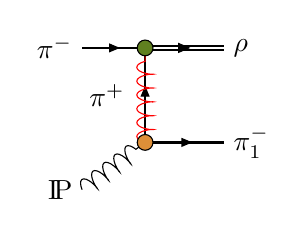
\begin{tikzpicture}[node distance=0.6cm and 0.8cm]
  \coordinate[] (z1);
  \coordinate[below =of z1] (a2);
  \coordinate[left=of a2, label=left:{$\mathrm{I\!P}$}] (a1);
  \coordinate[above =of z1] (z2);
  \coordinate[above=of z2] (b2);
  \coordinate[left=of b2, label=left:{$\pi^{-}$}] (b1);
  % \coordinate[right=of b2] (b2);
  \coordinate[      right=of b2,xshift=2mm,label=right:{$\rho$}] (b3);
  \coordinate[right=of z1,xshift=2mm,label=right:{$\pi_1^-$}] (b5);

  \draw[gluon]  (a1) -- node[] (a1z3) {} (z1);
  % \draw[]  (a1z3) to[out=-45, in=225, edge node={node[label={below, yshift=2mm}:{$t$}] {}}] (z3a3);
  % \draw[scalar]  (z1) to[out=135, in=225, edge node={node [label=left:{$\pi^+$}] {}}]  (b2);
  \draw[scalar]  (z1) -- node [label=left:{$\pi^+$}] {} (b2);
  \draw[gluon, red]  (z1) -- (b2);
  \draw[scalar]  (b1) -- (b2);
  \draw[vector]  (b2) -- (b3);
  \draw[scalar]  (z1) -- (b5);
  \node[circle,draw=black,fill=green!50!purple,inner sep=0pt,minimum size=2mm] at (b2) {};
  \node[circle,draw=black,fill=yellow!50!purple,inner sep=0pt,minimum size=2mm] at (z1) {};
  % \draw [decorate,decoration={brace,amplitude=3pt}] ($(b4)+(1.2,0.1)$) -- ($(b3)+(1.2,-0.1)$) node [black,midway,xshift=0.4cm] {$\sigma_1$};
  % \draw [decorate,decoration={brace,amplitude=3pt}] ($(b5)+(1.2,0.1)$) -- ($(a3)+(1.4,-0.1)$) node [black,midway,xshift=0.5cm] {$s_{p\pi_1}$};
  % \draw [decorate,decoration={brace,amplitude=3pt}] ($(a1)-(1.2,0.1)$) -- ($(b1)-(1.2,-0.1)$) node [black,midway,xshift=-0.4cm] {$s_0$};
  % \draw[thin,<-] ($(z1)+(-0.0,0.35)$) -- node[label={right,xshift=-1mm}:{$t_1$}] {} ($(b2)+(-0.0,-0.35)$);

\end{tikzpicture}
\end{document}
